\documentclass{article}
\usepackage{fancyhdr}
\usepackage{extramarks}
\usepackage{amsmath}
\usepackage{amsthm}
\usepackage{amsfonts}
\usepackage{tikz}
\usepackage[plain]{algorithm}
\usepackage{algpseudocode}

\begin{document}
\author{Chuan Lu}
\title{PHYS:5905 Homework 4}
\maketitle

\medskip

\begin{enumerate}
\item
Magnetic Mirror Confinement

\begin{enumerate}
\item Verify that $\nabla\cdot B = 0$ for this magnetic mirror field.

\begin{proof}
In fact, we only need to prove this for the normalized magnetic field $B'$.
$$
\begin{aligned}
\nabla\cdot B' &= \frac{\partial}{\partial x'}B_x'+ \frac{\partial }{\partial y'}B_y' + \frac{\partial }{\partial z'} B_z' \\
&= -\frac{\pi}{2L'}\delta B_z'\sin(\frac{2\pi z'}{L}) -\frac{\pi}{2L'}\delta B_z'\sin(\frac{2\pi z'}{L}) + \frac{2\pi}{2L'}\delta B_z'\sin(\frac{2\pi z'}{L'}) \\
&= 0.
\end{aligned}
$$
\end{proof}

\item 
For an initial position $x_0/r_L = (0.1, 0, 8)$, and initial velocity $v_0/v_\perp = (0, 1, 0)$, plot the trajectory of the particle on the $(z, x)$ plane over a simulation time $\Omega T = 10\pi$.

The trajectory is shown in Figure \ref{problem 1.1}.
\begin{figure}[h]
\centering
\vbox{
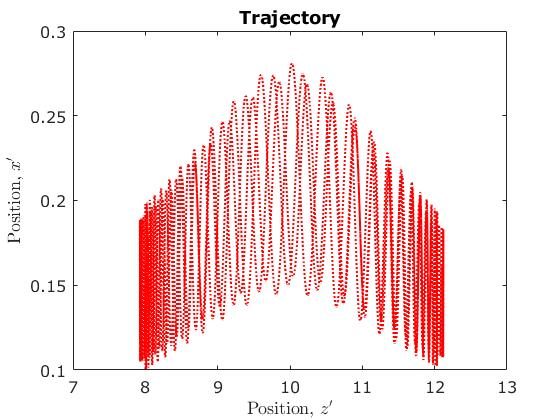
\includegraphics[scale=0.4]{problem4a/trajectory_zx_5000.jpg}
}
\caption{The trajectory in the $(z, x)$ plane with AB3 scheme and $N=5000$ timesteps, and final time $T' = 10\pi$.}
\label{problem 1.1}
\end{figure}

\item
Plot the 3D trajectory of the particle of the same simulation over plotted region.

The trajectory is shown in Figure \ref{problem 1.2}.
\begin{figure}[h]
\centering
\vbox{
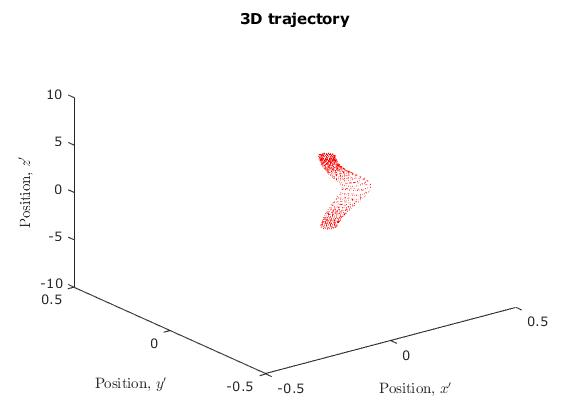
\includegraphics[scale=0.4]{problem4a/trajectory_3d_5000.jpg}
}
\caption{The trajectory in the $(x, y, z)$ plane with AB3 scheme and $N=5000$ timesteps, and final time $T' = 10\pi$.}
\label{problem 1.2}
\end{figure}

\item Plot the evolution of normalized magnetic moment.

The plot is shown in Figure \ref{problem 1.3}, where we observe that with the increase of timesteps $N$, the conservation gets better.

\begin{figure}[h]
\centering
\vbox{
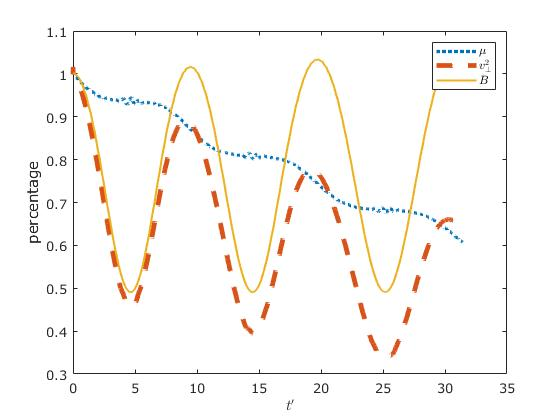
\includegraphics[scale=0.3]{problem4a/magnetic_5000.jpg}
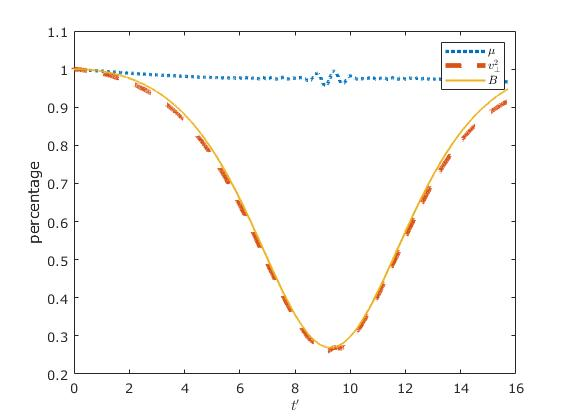
\includegraphics[scale=0.3]{problem4a/magnetic_10000.jpg}
}
\vbox{
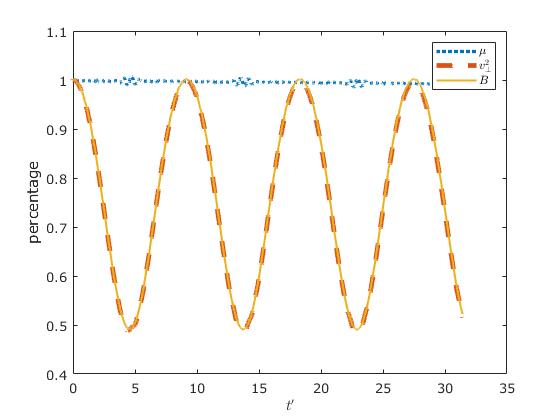
\includegraphics[scale=0.3]{problem4a/magnetic_20000.jpg}
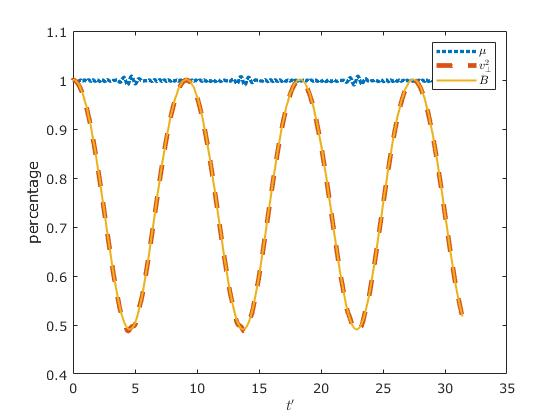
\includegraphics[scale=0.3]{problem4a/magnetic_50000.jpg}
}
\caption{The normalized magnetic moment $\mu$, normalized perpendicular velocity $v_\perp^2 $ and magnetic field magnitude $B$. Top: number of time steps $N = 5000, 10000$. Bottom: $N = 20000, 50000$.}
\label{problem 1.3}
\end{figure}

\item
Plot the evolution of normalized kinetic energy.

The plot is shown in Figure \ref{problem 1.4}, where we observe that with the increase of timesteps $N$, the conservation gets better.

\begin{figure}[h]
\centering
\vbox{
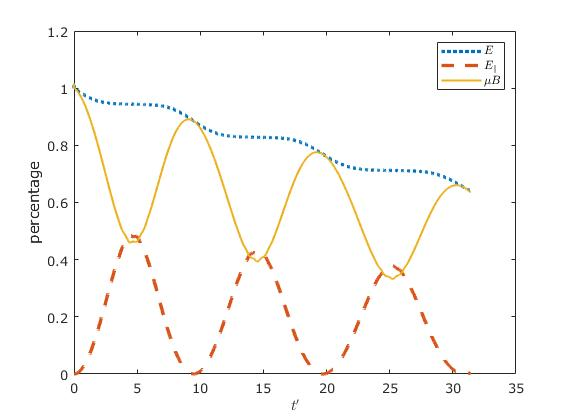
\includegraphics[scale=0.29]{problem4a/energy_5000.jpg}
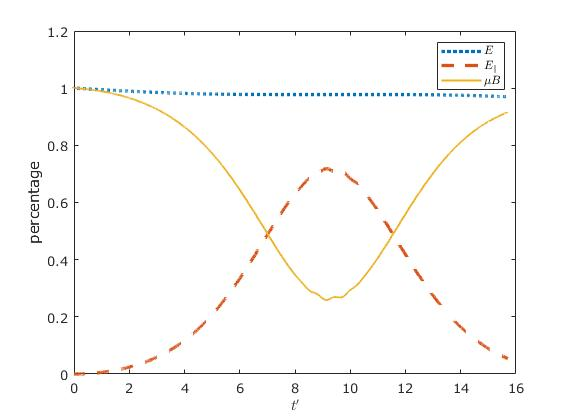
\includegraphics[scale=0.29]{problem4a/energy_10000.jpg}
}
\vbox{
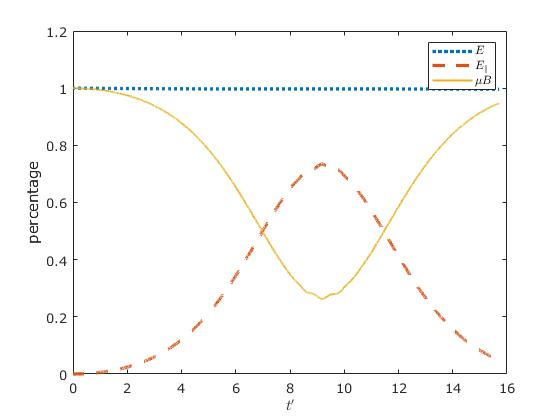
\includegraphics[scale=0.29]{problem4a/energy_20000.jpg}
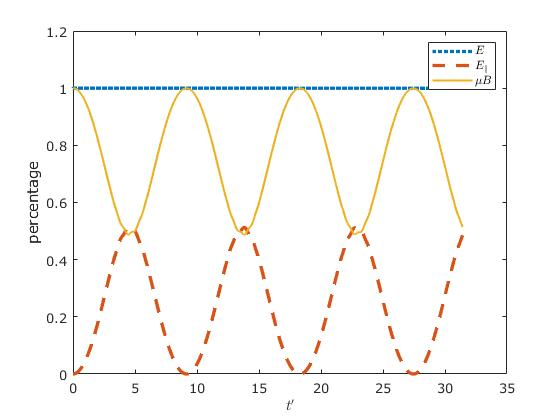
\includegraphics[scale=0.29]{problem4a/energy_50000.jpg}
}
\caption{The normalized total kinetic energy $E$, normalized parallel kinetic energy $E_\parallel $ and $\mu B$. Top: number of time steps $N = 5000, 10000$. Bottom: $N = 20000, 50000$.}
\label{problem 1.4}
\end{figure}

\end{enumerate}

\end{enumerate}


\end{document}